% ============================
% Extra 2
% ============================
%
\begin{tikzpicture}[x=1mm, y=1mm]
    \tikzmath{\fs = \textsize + 0.5;}
    
    % Parchment paper
    \draw[fill=parchment] (0,0) rectangle (63,88);
    
    % Imagem
    \node[anchor=north west, inner sep=0,outer sep=0] (image) at (0, 88) {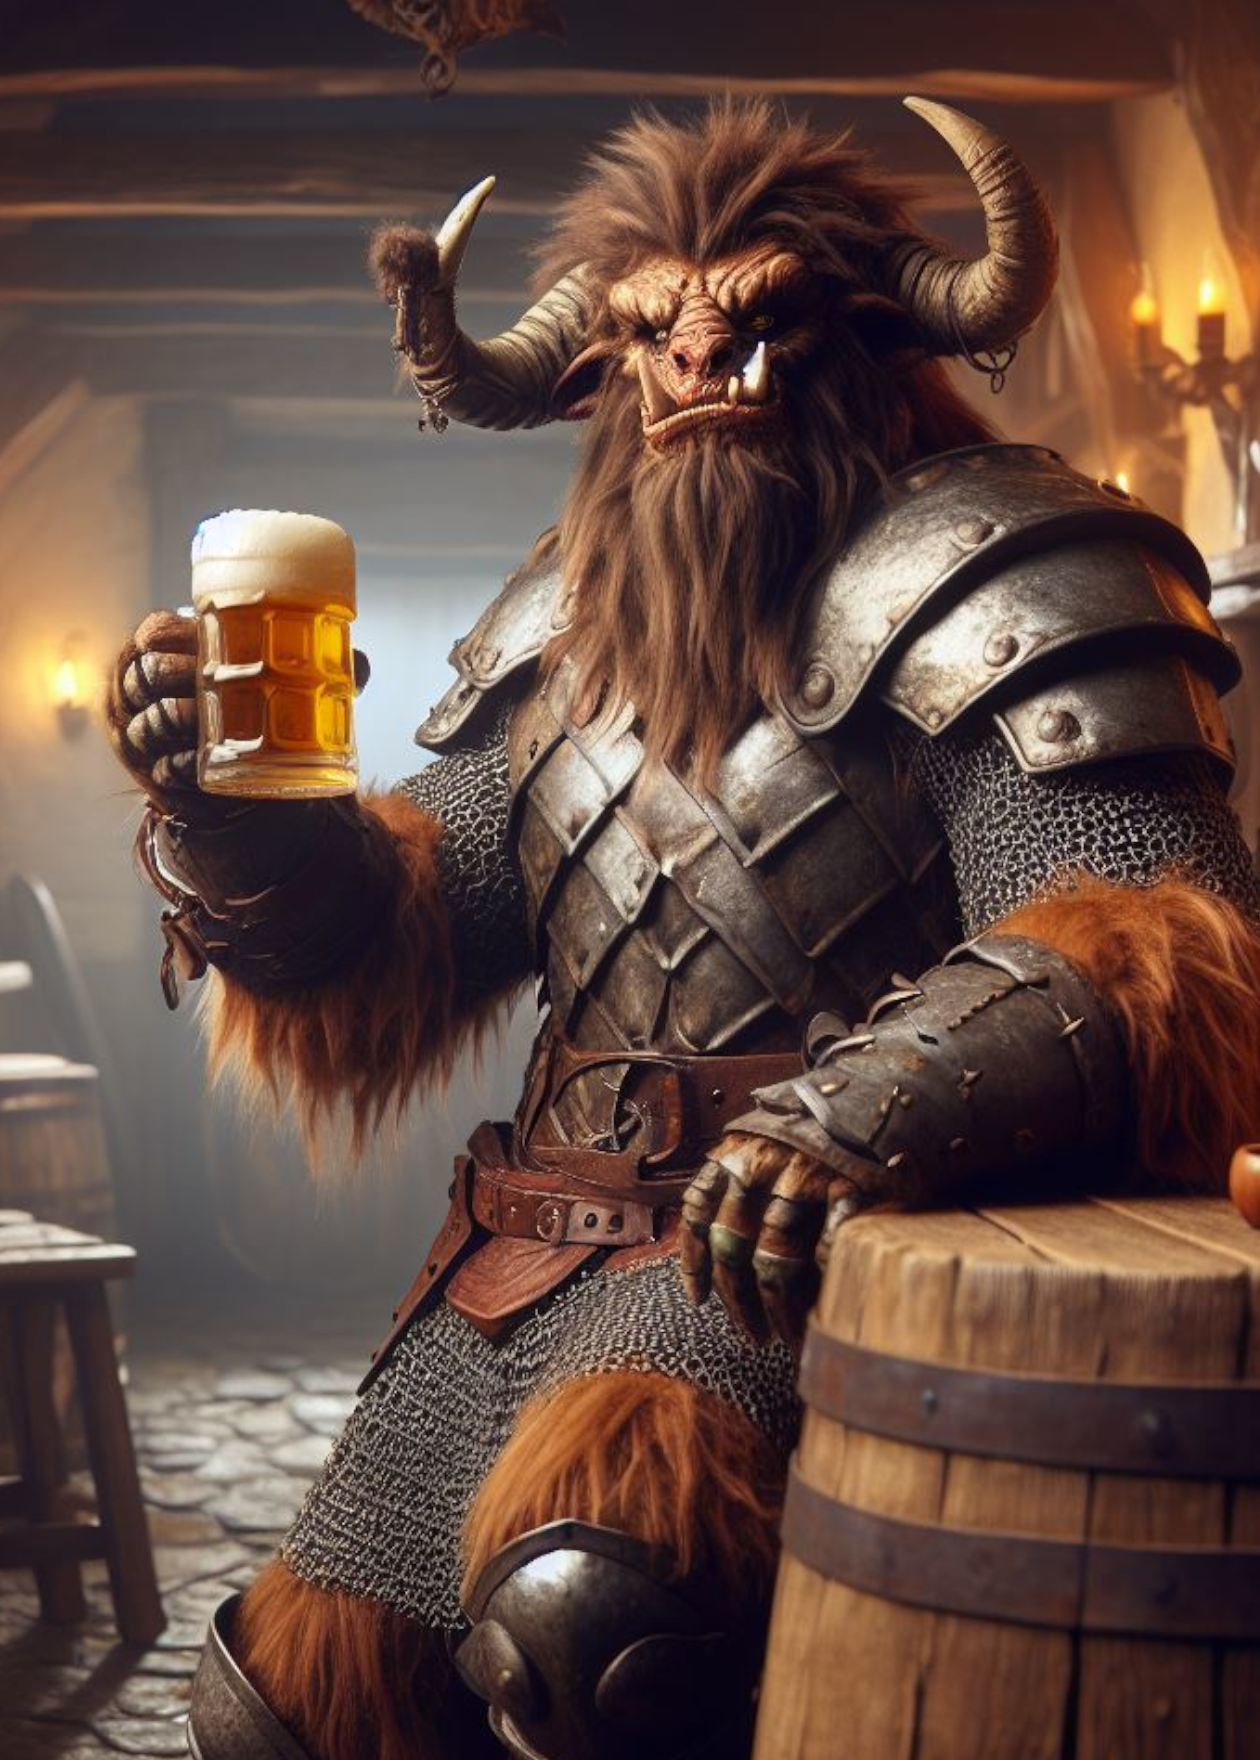
\includegraphics[width=63mm, height=88mm]{images/bugubi.png}};
    
    % Título
    \node[title, anchor=north west, minimum width=59mm](title) at (2,86) {Extra info - 2};
    

    % FIGHTER
    \node[fill=parchment, opacity=0.7, text opacity=1, draw opacity=1, inner sep=0mm, anchor=north west, font=\sffamily\fontsize{8}{8.5}, draw=black, rounded corners=0.4mm, fit={(2,80) (61,36)}] (FIGHTER) {};
    \node[tag, anchor=west] at ([xshift=0.5mm] FIGHTER.north west) {FIGHTER};
    \node[anchor=north west, align=justify, yshift=-1mm, text width=27mm, font=\sffamily\fontsize{4.5}{5}\selectfont] (bugbear) at (FIGHTER.north west) {%
    \textbf{Fighting Style:} You have honed your martial prowess and gain a Fighting style feat of your choice (great weapon fighting).\\[0.5em]\textbf{Great weapon fighting:} When you roll a 1 or 2 on damage die for an attack you make with a melee weapon that you arewielding with two hands, you can reroll the die, and you must use the new roll.\\[0.5em]The weapon must have the Two-Handed or versatile property to gain this benefit.\\[0.5em]
    \textbf{Weapon mastery:} Your training with weapons allows you to use the mastery property of three kinds of simple or martial weapons of your choice.\\[0.5em]Whenever you finish a long rest, you can practice weapon drills and change one of those weapon choices.\\[0.5em]Weapons: Halberd, pike and hand axe\\[0.5em]
    };
    
    \node[anchor=north west, align=justify, yshift=-1mm, text width=28mm, font=\sffamily\fontsize{4.5}{5}\selectfont] (bugbear) at ([xshift=28mm] FIGHTER.north west) {%
    \textbf{Pole Strike:} Immediately after you take the Attack Action and attack with a Weapon that has the Heavy and Reach properties, you can use a Bonus Action to make a Melee Attack with the opposite end of the Weapon. The weapon’s damage die for this attack is a d4, and it deals Bludgeoning Damage.\\[0.5em]
    \textbf{Reactive Strike:} While you are holding a Weapon that has the Heavy and Reach properties, you can use your Reaction to make one Melee Attack against a creature\\[0.5em]
    \textbf{Tactical Shift:} Whenever you activate your Second Wind with a Bonus Action, you can move up to half your Speed without provoking Opportunity Attacks.\\[0.5em]
    };
    
    % EMPTY
    % \node[fill=parchment, opacity=0.7, text opacity=1, draw opacity=1, inner sep=0mm, anchor=north west, font=\sffamily\fontsize{8}{8.5}, draw=black, rounded corners=0.4mm, fit={(2,50) (61,2)}] (FIGHTER) {};
    % \node[tag, anchor=west] at ([xshift=0.5mm] FIGHTER.north west) {NOTES};

    % Borda
    \draw[line width = 0.5mm, black] (0,0) rectangle (63,88);
    
    \end{tikzpicture}%%